\documentclass[12pt]{article}
\usepackage{amsmath}
\usepackage{graphicx}
\usepackage{hyperref}
\usepackage{algorithm}
\usepackage{algpseudocode}
\usepackage{array} % for tables by HCJ
\usepackage{amsfonts} % added by HCJ
\graphicspath{ {./images/} }
\usepackage[a4paper, total={8in, 10in}]{geometry}
\usepackage[latin1]{inputenc}

\title{MATH4995 Final Project: Pawpularity Prediction}
\author{CHOW, Hau Cheung Jasper}
\date{1 November 2021}

\begin{document}
\maketitle

\section{Background}
Stray animals pose significant health and environmental risks as they can attract predators into suburban residential areas and potentially carry disease [1]. Many organisations have thus taken it upon themselves to adopt strays and supply them to loving families in need of companionship. However, one of the biggest hurdles faced by these animal welfare groups is the typical lack of funding and trained staff to manage such large animal populations, so the more stray animals that find homes faster, the better. Petfinder.my is one such organisation, and their current basic algorithm ranks the "Pawpularity" of pet photos for prospective adopters based on various metrics such as traffic data across web and mobile devices, but their algorithm is quite rudimentary. In this project, we will attempt to analyze the raw images and metadata of thousands of pet profiles to predict the Pawpularity of pets in an attempt to alleviate the burden on animal welfare groups and help stray dogs and cats find caring families, creating a win-win scenario.

\section{Data overview}
The data comes in two forms; namely a set of 9912 images and their corresponding metadata stored in "train.csv". Each raw image is a JPEG file in RGB format with a unique name called its 'Id', and can come in a variety of sizes and aspect ratios.

\subsection{Metadata}

Each image 'Id' has a corresponding row in "train.csv" which also holds values of certain metadata features of that image, such as 'Face' (whether or not the animal face is clear) and 'Action' (whether or not the animal is in the middle of an action like playing or jumping), as well as the image's \textbf{pawpularity score} (our desired response variable which ranges from $\{1,2,...,100\}$). Excluding the pawpularity score, there are 12 such features, each of which take a binary value. The dimensions of 'train.csv' are: 9912 x 14\newline

\noindent A constraint of the project is that submissions must be made through notebooks and the GPU runtime must not exceed 9 hours. Therefore, it is important not to overcomplicate our models and some tests that I have conducted will not be shown in the notebook and only in this report. The metric used to compute the model's goodness-of-fit is the \textbf{Root Mean Squared Error}: $RMSE=\sqrt{\frac{1}{n} \sum_{i=1}^{n} (y_i - \hat{y}_i)^2}$ where $y_i$ denotes the actual pawpularity score (hereafter referred to as 'score') of pet profile $i$ and $\hat{y}_i$ denotes the predicted score of pet profile $i$.

\section{Project methodology and pipeline}

The general structure of the project is as follows:

\noindent 1. Exploratory data analysis of the metadata (Section 4)\newline
2. Experiment with simple models to predict score from metadata alone (Section 5)\newline
3. If metadata is insufficient, build models to predict score from raw images (Section 6)\newline

The reason we attempt simple models first is the ease of interpretability. In the future, if additional metadata features are introduced, the model can be easily retrained to incorporate the new predictor. Furthermore, the regression coefficients of linear models correspond to the pawpularity score increase associated with having that feature, so by examining the regression equation, we can easily see which features contribute most to the Pawpularity score.

\section{Exploratory data analysis}

First, we observe there are no missing values in the "train.csv" metadata. As such, no data imputation is required.\newline

Second, we plot the histogram of the Pawpularity scores observed in the training dataset. We observe that the distribution is right-skewed and the peak appears to be in the 20-40 score range. This suggests that our model may perform poorly if the test distribution has more datapoints in the relatively underpopulated 60-90 range.
\begin{figure}[h]
\caption{Histogram of pawpularity scores (x=Scores, y=Number)}
\centering
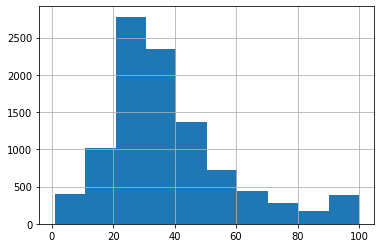
\includegraphics[scale=0.4]{1_pawpularity}
\end{figure}

We also observe the correlation heatmap for the 12 features and notice that no single feature appears to have good correlation with the response variable Pawpularity. The most notable correlations are between Human/Occlusion (0.63), Info/Collage (0.48), Face/Eye (0.58), Group/Near (-0.32) and Blur/Eyes (-0.51).
\begin{figure}[h]
\caption{Pairwise correlation heatmap of features}
\centering
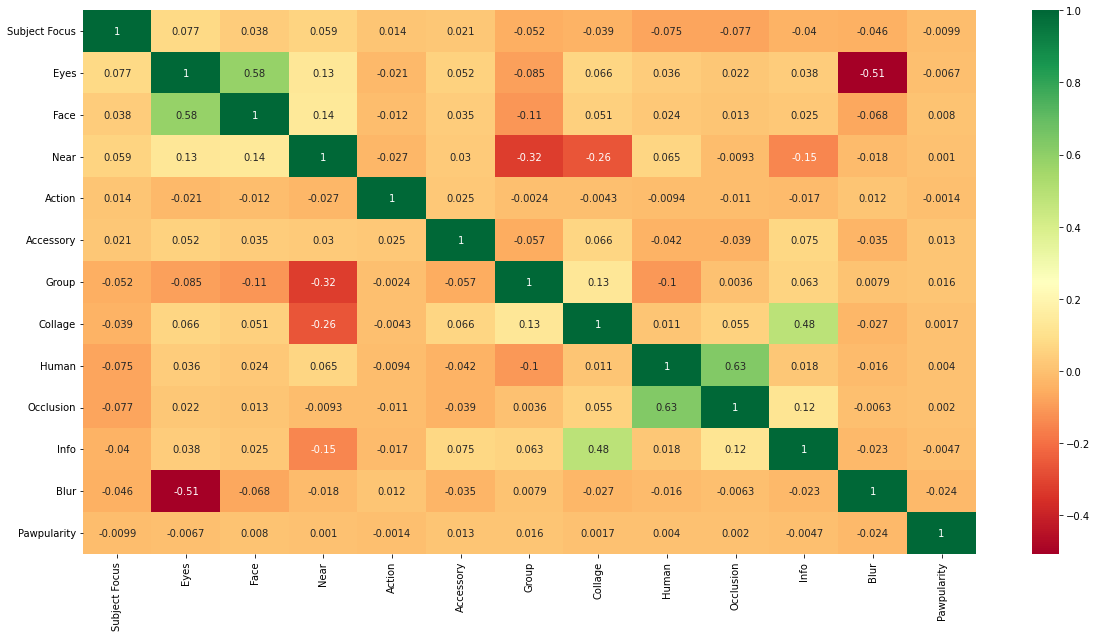
\includegraphics[scale=0.3]{2_correlation}
\end{figure}

When conducting regression, we must check to see that multicollinearity assumptions are not violated; if they are, the regression coefficients lose their interpretability. Therefore, we calculate the Variance Inflation Factor of each predictor; defined as $VIF_{i}=\dfrac{1}{1-R^{2}(X_i)}$ where $R^{2}(X_i)$ denotes the multiple $R^2$ of predictor $X_i$ against all other predictors (i.e. the proportion of variability of predictor $X_i$ that could be explained by the other predictors.) In general, $VIF_{i}\geq10$ indicates multicollinearity and we should remove predictor $i$.\newline

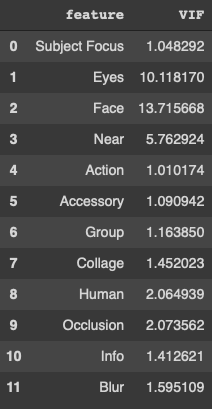
\includegraphics[scale=0.4]{7_VIF}

In this case, we observe that indeed both 'Eyes' and 'Face' predictors have $VIF\geq 10$. Therefore, we choose to remove the feature 'Eyes' since it has strong negative correlation with another feature 'Blur'. We also use principal component analysis (PCA) to determine the optimal number of features in our predictive model and find that 9-10 features can preserve over 90\% of the variance, so indeed one or two features can be dropped.\newline

We also run some exploratory plots on each of the predictors to see how they are distributed. We separated the possible pawpularity scores into 10 quantiles (one quantile from 1-10, one quantile from 11-20, etc.) and since all the predictors are indicator variables, we plotted the frequency of each predictor for each score quantile.\newline

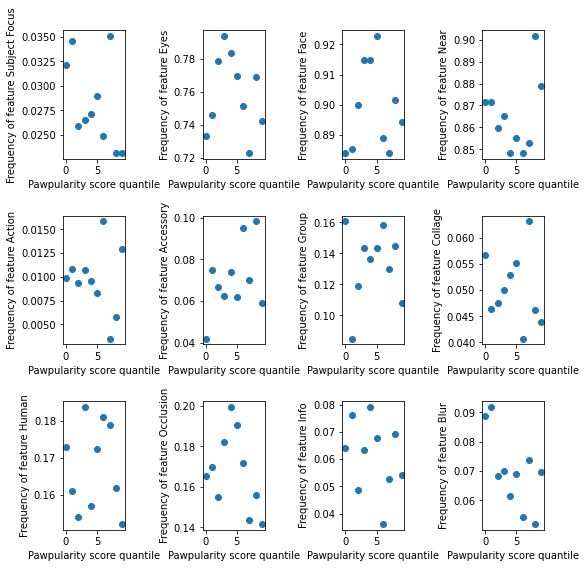
\includegraphics[scale=0.4]{3_predictorsvquantile}

Overall, there does not appear to be any noticeable trends of any predictor with the score value; i.e. each score band has roughly the same proportion of that predictor. Some predictors have low frequencies at every score quantile, such as 'Subject Focus', where the proportion of pets that have it range between 0.025 and 0.035.

\section{Experiment - prediction on metadata}

\subsection{Simple regression models}

Firstly, we attempt to use (i) \textbf{logistic regresion} (treating the problem as a 100-class classification problem), (ii) \textbf{linear regression}, (iii) \textbf{ElasticNet regression} (i.e. linear regression with both $L_1$ and $L_2$ norm penalties), (iv) \textbf{decision tree regressor}, and (v) \textbf{random forest regressor} (with decision tree regressor as base classifier.) Our 5-fold cross validation RMSE results are shown below.\newline

\begin{center}
\begin{tabular}{ | m{1.2cm} | m{3cm}| m{3cm} | m{2cm} | m{3cm} | m{3cm} | } 
  \hline
  Method & Logistic Regression & Linear regression & ElasticNet & Decision Tree regressor & Random forest regressor with \texttt{n\_estimators=50}\\ 
  \hline
  RMSE & 23.386 & 20.600 & 20.589 & 20.854 & 20.763 \\ 
  \hline
\end{tabular}
\end{center}

We also did some additional work with the Decision Tree regressor by using grid search on the pruning parameter $\alpha$ by sampling 50 equally spaced values in the interval $[10^{-6}, 10^{-1}]$. We ended up finding $\alpha=0.1$ to be the parameter value with the best 5-fold cross-validation MSE. The pruned decision tree yielded a 5-fold RMSE of \textbf{20.666} (slight improvement) and is as follows:

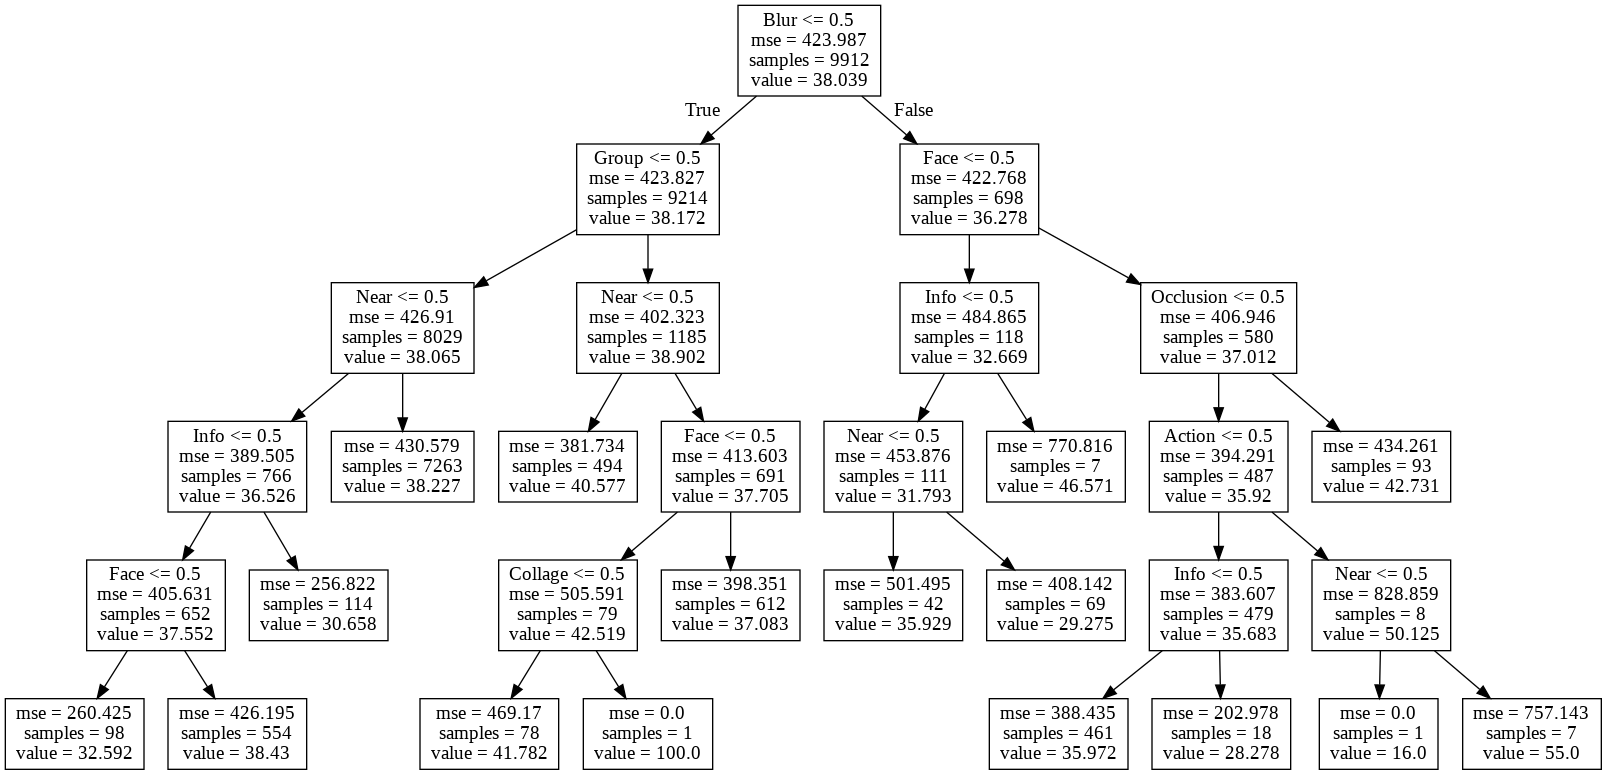
\includegraphics[scale=0.2]{4_prunedtree}

In our random forest regressor, we also evaluated the importance of each of the features in the model and found the most significant features were:

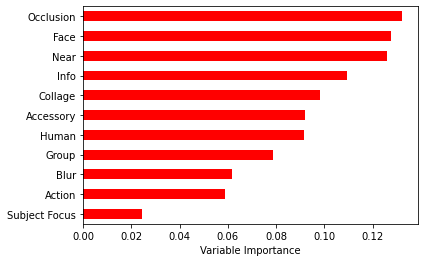
\includegraphics[scale=0.4]{6_feature_importance}

We listed out and gradually dropped features in the random forest model starting with the least important ones (keeping the top 5 most important features), then found the lowest mean 10-fold CV RMSE for each subset of features and considered the smallest subset of features within 1SD of that value. Our 5-fold cross-validation mean RMSE was \textbf{20.630} (slight improvement) with the features \{Occlusion, Face, Near, Info, Collage\}.\newline

In summary, we see that logistic regression performed the poorest (without even taking into account the class imbalance, since many scores are in the 20-40 range), followed by random forest and decision tree with similar performance. ElasticNet regression and simple linear regression had the lowest 5-fold mean cross-validation RMSE, though we observe that the slight decrease in RMSE in ElasticNet regression is likely negligible. Further experiments with the random forest also showed that increasing the number of estimators \texttt{n\_estimators} for random forest to 300 did not improve the 5-fold mean RMSE score by a significant amount.

\subsection{Ordinal regression}

When researching some ways to limit the output of these simple models to a fixed interval $[1,100]$, I came across the idea of \textbf{ordinal regression}. It is defined as learning a classifier $h:\mathcal{X} \rightarrow \mathcal{Y}$ from data $(X_1,Y_1),...,(X_n,Y_n)$ where $X_i\in \mathcal{X}$, $Y_i\in \mathcal{Y}=\{1,2,...,k\} \forall i\in \{1,...,n\}$ such that the average loss $L$ over all $(X,Y)$ pairs  (i.e. $\mathbb{E}_{X\times Y}[L(Y,h(X))]$) is minimised. [2]\newline

Ordinal regression differs from the standard multiclass classification in that the 0-1 loss is not sensitive to the distance among target values. For instance, in cross-entropy, if a picture is of a dog, it doesn't matter if we misclassify it as a spider or as a cat - either is equally wrong. But in ordinal regression, as there is an 'order' between labels, the loss function becomes lower as the between-class 'distance' decreases. If we were to apply ordinal regression, we might consider that a dog is closer to a cat than a spider, and hence the cat would be a 'less incorrect' prediction. Since our model is evaluated via RMSE, misclassifying a pawpularity score of $p$ as $p+1$ should be penalised less than $p+2$. Hence, we attempt to fit two variants of ordinal regression to our metadata: (i) linear ordinal ridge regression (with L2 penalty), and (ii) logistic ordinal regression. The models were implemented with the \texttt{mord} library and the 5-fold mean RMSE scores are:\newline

\begin{center}
\begin{tabular}{ | m{1.2cm} | m{5cm}| m{6cm} | } 
  \hline
  Method & Ordinal Logistic Regression & Ordinal LASSO regression \\ 
  \hline
  RMSE & 21.182 & 20.601 \\ 
  \hline
\end{tabular}
\end{center}

We can see that the ordinal regression method shows significant improvement only for the logistic regression approach. This suggests there may be a limit to the predictive strength of the metadata towards the pawpularity score and we should turn to the raw image data.

\section{Experiment - prediction on raw images}

\subsection{CNN architecture design}

The most typical method for extracting features from raw images is the convolutional neural network. By sliding a rectangular matrix called a \textbf{kernel} over the pixels of the image, abstract features can be extracted, and model weights are recomputed using backpropagation. Instead of building an architecture from scratch, we opt to use the preexisting ResNet architecture that have been proven to perform well. Furthermore, manually designed CNNs are more prone to bugs, have no theoretical evidence to support claims that they perform better than the well-known architectures, generally take more time to converge and train, and performance may be poorer, whereas ResNet models pretrained on ImageNet classification is readily available.\newline

The ResNet architecture was selected over AlexNet and VGG due to its \textbf{skip connections}, which prevent the vanishing/exploding gradient problem that causes early layers to update extremely slowly. It does so by causing gradient to pass through multiple layers (the Conv blocks) without any change in magnitude. The ResNet-50 architecture is given below, and we only added dropout, batch normalization, linear layers with an output size of 1 and a sigmoid since we want to predict the score.\newline

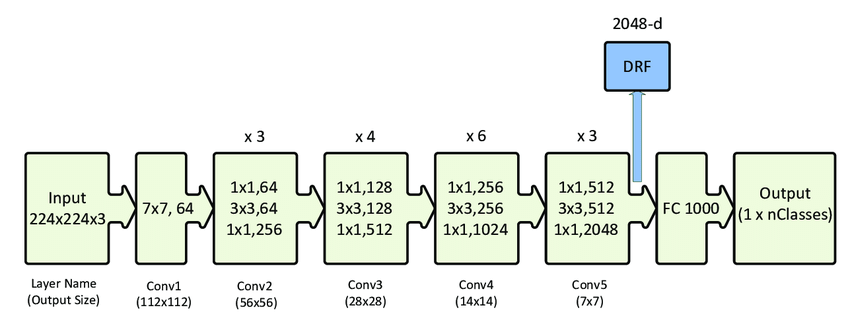
\includegraphics[scale=0.3]{5_resnet50}

Dropout and batch normalization were incorporated into this layer to lower generalisation error rates on the test set. During training, a dropout unit zeroes the output of a given neuron randomly with probability $p$, and as neurons become unreliable, the network is able to learn various independent representations of the network that may have been overlooked without dropout. Batch normalization is also used to convert the batched outputs between layers into a form with zero mean and unit variance, leading to increased network speed and stability. Finally, a sigmoid unit was included at the end to map the real-valued output into a value in the interval. $[0,1]$ as the pawpularity scores $[1,100]$ will also be scaled to this range. Alternative functions that map to $[0,1]$ could be used here, such as \texttt{tanh} or \texttt{softsign}.\newline

The motivation for our configuration comes from Srivastava et al. [5], which show that dropout combined with L2 regularization (\texttt{weight\_decay}) along with high momentum yield excellent performance.

\subsection{Preprocessing}

Since we are testing the 'cuteness' of an animal, any significant cropping, random erasure, blur, or colour jitter is likely to have an adverse and unpredictable effect on the score. As such, our data augmentation is limited to only horizontal flips, which we conduct on-the-fly with probability 0.5. All images are also resized to $224\times 224$ since they come in varying input dimensions, and the pixels in each input channel of each image are normalized with mean (0.485, 0.456, 0.406) and standard deviation (0.229, 0.224, 0.225).

\subsection{Training}

The dataset was randomly split into a training set consisting of 7912 images and validation set consisting of the remaining 2000 images, and the model was then trained on the training set for 20 epochs (with early stopping if validation set RMSE failed to improve for 4 epochs) Colab's free GPU with \texttt{batch\_size=32} and the SGD optimizer with \texttt{momentum=0.9} and L2 regularization \texttt{weight\_decay=0.001}. The loss function used was the mean-squared-error (MSE) loss. The standard dropout value of $p=0.5$ was used. Various learning rates were tested (since too large learning rates may cause the model to skip over certain parameter values, while low learning rates mean training time takes too long) and the best validation RMSE scores are given below. Note that the training and validation sets have roughly the same proportion of pets (stratification) in each score band.\newline

\begin{center}
\begin{tabular}{ | m{3.4cm} | m{4cm}| m{4cm} | m{4cm} | } 
  \hline
  Model/Parameters & \texttt{learning\_rate=0.01} & \texttt{learning\_rate=0.001} & \texttt{learning\_rate=0.0001}\\ 
  \hline
  ResNet-18 & 21.1673 & 18.5846 & 18.6221 \\
  \hline
  ResNet-50 & 19.8544 & 17.9965 & 18.0132 \\ 
  \hline
\end{tabular}
\end{center}

As training is computationally-intensive, grid search of hyperparameters such as regularization coefficient $\alpha$ and momentum were not used, nor was k-fold cross-validation.\newline

We can see that the best learning rate appears to be 0.001. The model converges relatively quickly to a validation RMSE of 17.9965 for ResNet-50 in 14 epochs. It can be shown that increased depth does improve the performance slightly, but it is unclear if even deeper ResNets will perform better, and we also have to consider how deeper networks will take even longer to train as there are more parameters to update. The model performs slightly better than the simple regression and tree-based models tried in Section 4.

%\subsection{Visualisation}

%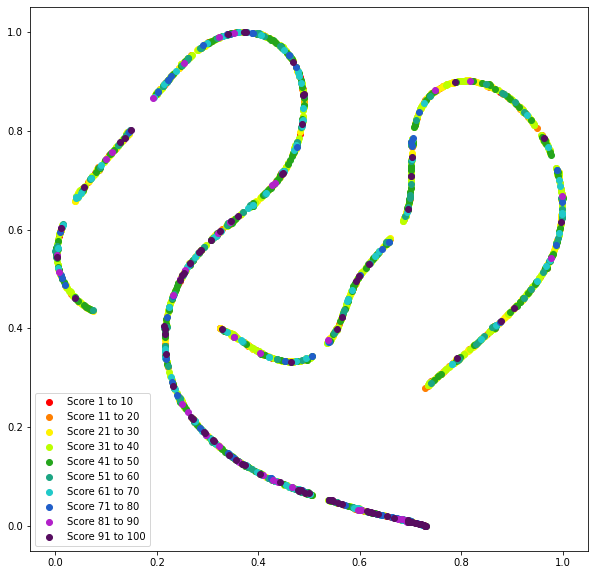
\includegraphics[scale=0.4]{10_TSNE}

%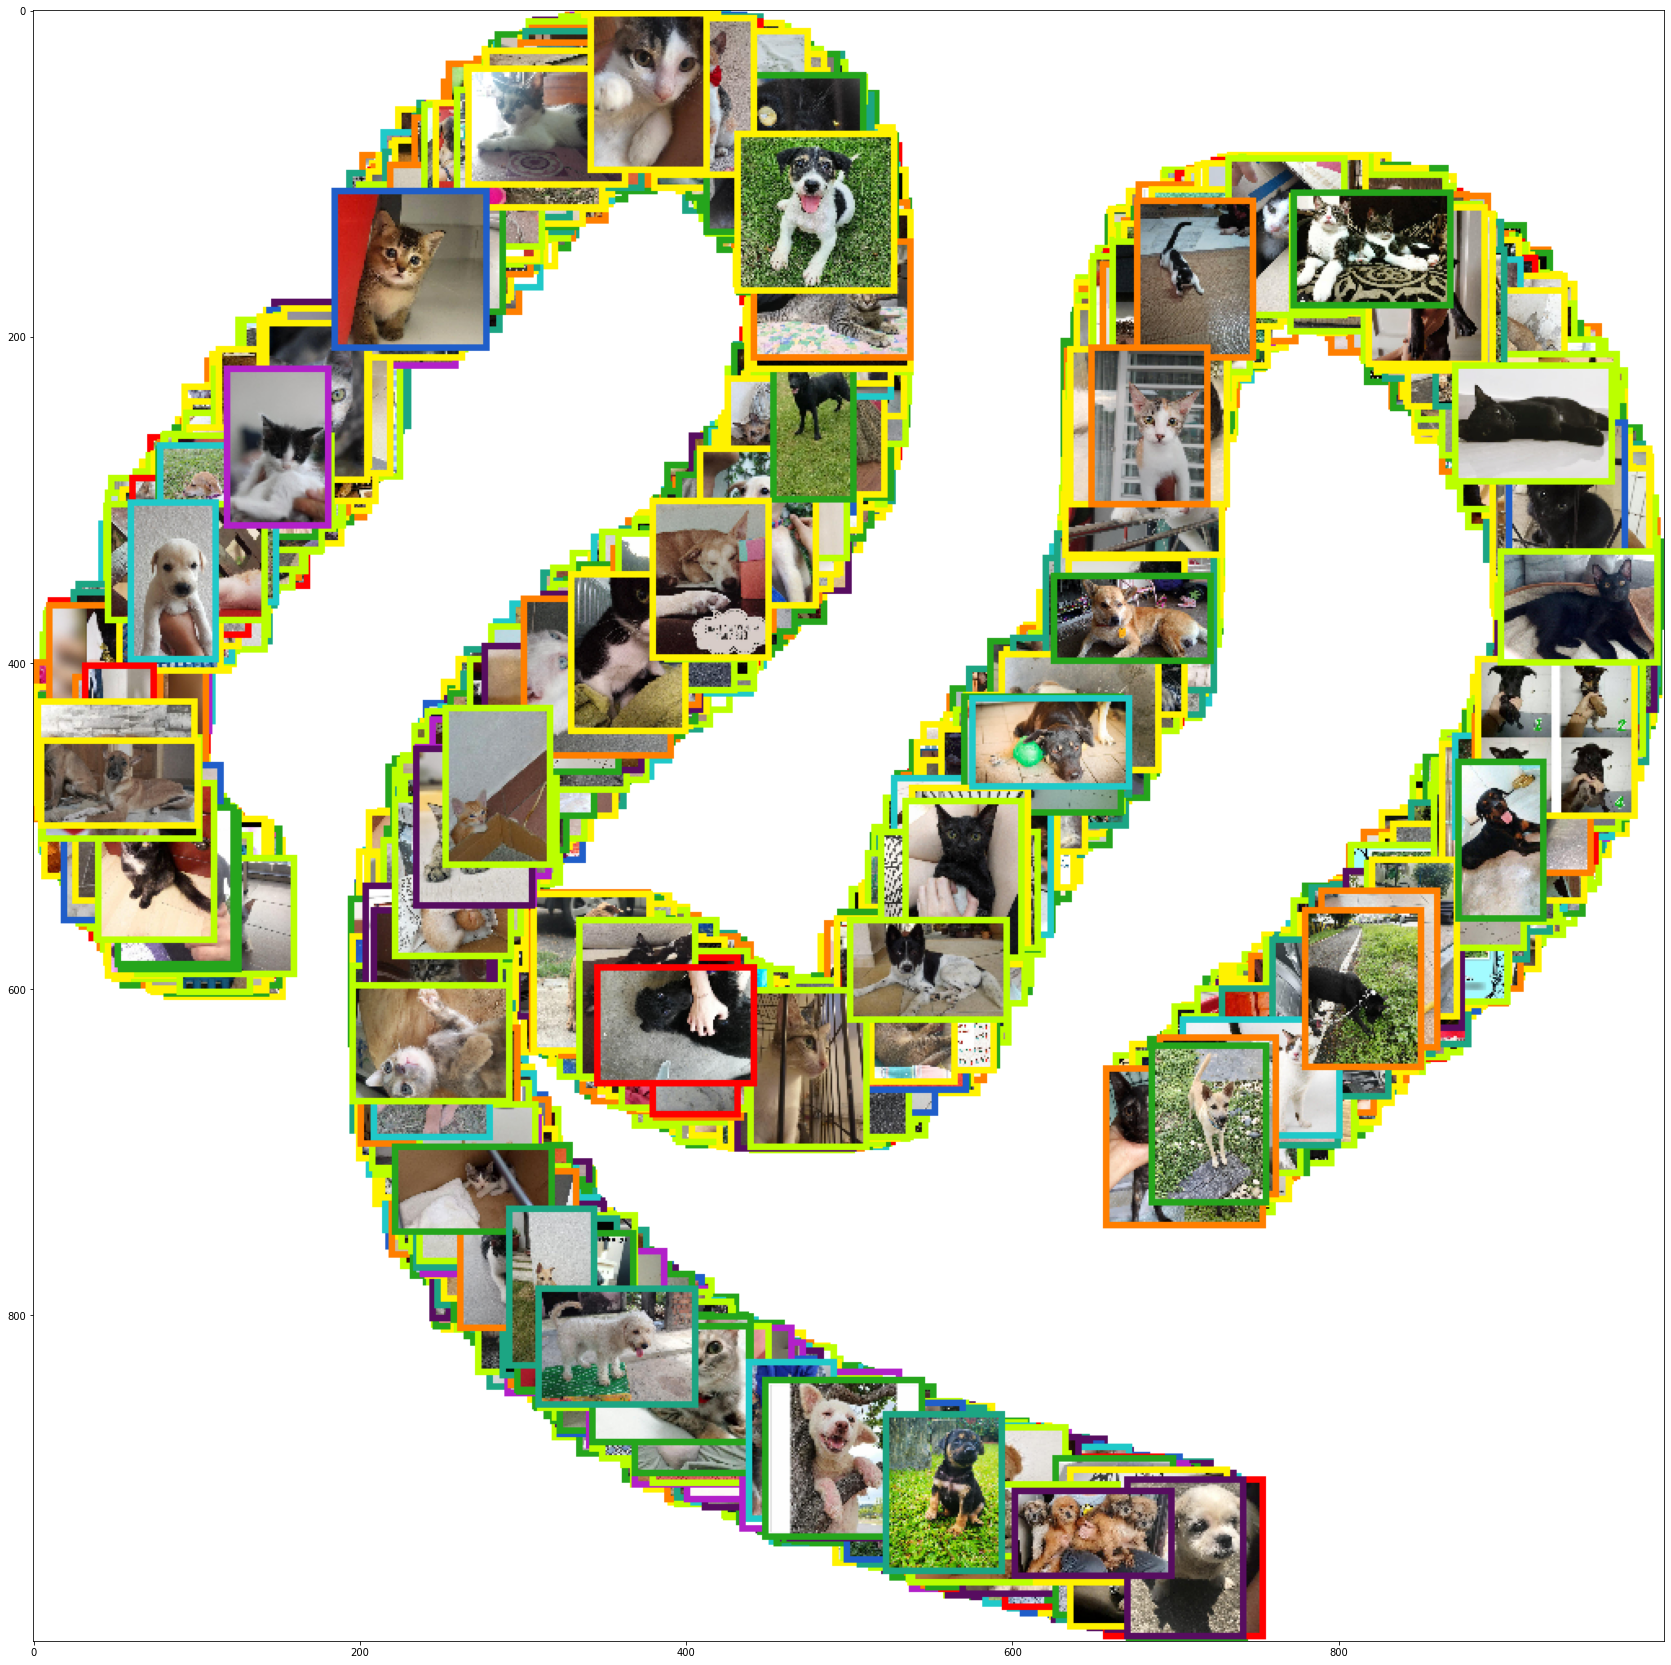
\includegraphics[scale=0.2]{9_TSNE}

%tSNE (t-distributed Stochastic Neighbour Embedding) was used to graphically visualise (in 2-dimensions) the differences in certain images. Warmer colours (red, orange, yellow) indicate lower pawpularity scores, while cooler colours indicate higher ones, with purple being the 91-100 score band. We can see there are 5 main clusters and that the main concentration of purple dots (high pawpularity) corresponds to many pale-coloured dogs and close up shots.

\subsection{Improving the loss function}

As our validation set was stratified to be similarly distributed to the training set and hence as a large proportion of pets in the 30-40 score range, to further improve our model generalizability, we constructed a \textbf{distribution-aware (weighted) RMSE loss} function in accordance with the \textbf{label-distribution-smoothing} approach recommended by Yang et al. [3]. From our training set, we would compute the average proportion of each score band in the training set, and use its inverse to weight the RMSE loss.\newline

Let $p_i$ $\forall i \in \{0,...,9\}$ denote the proportion of pets with scores in range $[10i+1,10(i+1)]$. Let $m=max\{p_0,...,p_9\}$. Our weighted RMSE loss is $RMSE_{weighted}=\sqrt{\frac{1}{n} \sum_{i=1}^{n} \dfrac{m}{p_i}(y_i - \hat{y}_i)^2}$.\newline

Similar to the LDAM loss used in classification of imbalanced datasets [4], our new loss function would cause the model to heavily penalize RMSE of rarely seen score bands (60-80 range) ensuring that the model does not largely learn to predict the most common score values in the 30-40 range. After training our model with this new loss function (again with dropout value $p=0.5$), our best validation RMSE scores are:

\begin{center}
\begin{tabular}{ | m{3.4cm} | m{4cm}| m{4cm} | m{4cm} | } 
  \hline
  Model/Parameters & \texttt{learning\_rate=0.01} & \texttt{learning\_rate=0.001} & \texttt{learning\_rate=0.0001}\\ 
  \hline
  ResNet-50 & 17.1055 & 13.3793 & 13.6822 \\ 
  \hline
\end{tabular}
\end{center}

We denote Model A and Model B to be the ResNet-50 with \texttt{learning\_rate=0.001} and loss functions MSE and weighted RMSE respectively. Model B is a significant improvement over Model A!

\section{Final model}

\begin{center}
\begin{tabular}{ | m{5cm} | m{3cm}| m{3cm} | } 
  \hline
  Model & Model A & Model B \\ 
  \hline
  Kaggle test RMSE & 20.45210 & 19.11171 \\ 
  \hline
\end{tabular}
\end{center}

Our Kaggle test RMSE is unfortunately not that good despite the otherwise leaderboard-topping validation RMSE results, indicating that the distribution of the test set is likely wildly different compared to the given data. Therefore, we decided to tinker with other CNN structures and see if they would provide better results, and chose the EfficientNet structure as it can be easily scaled up and its performance on the CIFAR-100 dataset is comparable to that of ResNet-50.\newline

EfficientNet conducts grid search to find the relationship between different scaling dimensions of the baseline network under some resource constraint and determines a compound scaling coefficient for each dimension. This method has been shown to improve model accuracy and efficiency compared to conventional scaling methods (i.e. ResNet). A neural architecture search is also used to determine a "good" framework, and EfficientNet largely relies on the \textbf{mobile inverted bottleneck convolution (MBConv) block} [6], which divides the original convolution into a depthwise and then a pointwise convolution to reduce computational cost with minimal accuracy loss. MBConv also uses a linear bottleneck in the final layer of each block to prevent loss of information from the ReLU unit. The EfficientNet structure is given below, and we only added BatchNormalization, Dropout, and two Dense layers to the last layer:

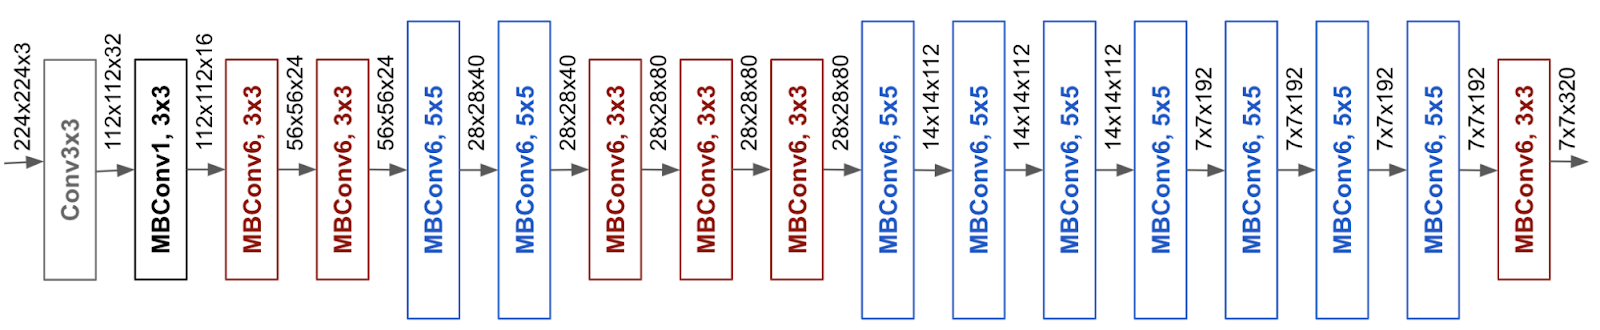
\includegraphics[scale=0.3]{8_efficientnet}

This model (Model \textbf{C}) was trained for 20 epochs with Adam optimizer (since Adam generally converges faster than SGD), initial \texttt{learning\_rate=0.001} with decay rate of 0.98 at each epoch, the MSE loss, dropout $p=0.2$, and early stopping with patience of 5. Model C achieved a validation RMSE of \textbf{14.8244}. Unlike our previous ResNet models, we could see that both the loss function and the model's validation RMSE is continuing to decrease at a steady pace even after the 20th epoch, which suggests that the model could continue to be trained until the validation RMSE starts to stagnate.\newline

Nevertheless, due to time constraints, Model C was submitted to Kaggle and achieved a \textbf{test RMSE of 18.04416} which is a significant improvement on the prior models.

\section{Future research}

Although the metadata is given in both the training and test datasets, they were manually labeled. Although predicting the score of the raw image is useful, it may be more helpful if we are able to extrapolate which features are the most associated with Pawpularity, since that can inform PetFinders how to take pictures that are more likely to be popular. Therefore, a CNN could be built to extract a $12\times 1$ feature vector from each image corresponding to the metadata.\newline

Additionally, the pawpularity score itself is not solely influenced by photo composition, but rather the specific animal in that picture. Certain users may have a preference for certain breeds of animals, so if the information is available, incorporating information such as cat/dog breed, age, gender and disposition instead of a single "Info" variable may provide further opportunities for enhancing performance.\newline

A more rigorous search of the hyperparameter space could be used to further finetune model performance, as well as selecting from different optimizers (i.e. Adagrad, RMSprop), different values of \texttt{weight\_decay} and the dropout parameter $p$. Finally, ensembling CNNs by training each of them on subsets of the entire given data and averaging their predictions could be used to improve generalization.

\section{Conclusion}

It is likely that EfficientNet as an overall structure may be more suitable to this problem compared to ResNet due to its better performance on the test set. Linear and tree-based models based on the metadata alone are likely too simplified to provide any meaningful insight. However, the metadata inputs could potentially be concatenated with the CNN output at some stage and combining both forms of input data has yield even better results (on the public leaderboard, one individual did this with Rapids-SVR to achieve test RMSE of 17.8.)

\section{Bibliography}

[1] Turner, Berry and MacDonald. "Animal shelters and animal welfare: raising the bar." 2012.\newline
https://www.ncbi.nlm.nih.gov/pmc/articles/PMC3398531/\newline
[2] Fabian Pedregosa-Izquierdo. "Feature extraction and supervised learning on fMRI: from practice to theory." Medical Imaging. Universite Pierre et Marie Curie - Paris VI, 2015. English. NNT: 2015PA066015. tel-01100921v2. Retrieved from: https://tel.archives-ouvertes.fr/tel-01100921v2/document\newline
[3] Yang, Zha, Chen, Wang, Katabi. "Delving into Deep Imbalanced Regression." https://arxiv.org/abs/2102.09554\newline
[4] Cao, Kaidi, Colin Wei, Adrien Gaidon, Nikos Arechiga, and Tengyu Ma. "Learning imbalanced datasets with label-distribution-aware margin loss." In Advances in Neural Information Processing Systems, pp. 1565-1576. 2019.\newline
[5] Srivastava, Hinton, Krizhevsky, Sutskever and Salakhutdinov. "Dropout: A Simple Way to Prevent Neural Networks from Overfitting." https://jmlr.org/papers/v15/srivastava14a.html\newline
[6] Tan, Le. "EfficientNet: Improving Accuracy and Efficiency through AutoML and Model Scaling." 29 May 2019. https://ai.googleblog.com/2019/05/efficientnet-improving-accuracy-and.html

\end{document}